\documentclass[10pt,a4paper,twocolumn,twoside]{article}
\usepackage[utf8]{inputenc}
\usepackage[english]{babel}
\usepackage{graphicx}
\usepackage{fancyhdr}
\usepackage{times}
\usepackage{titlesec}
\usepackage{multirow}
\usepackage{lettrine}
\usepackage[top=2cm, bottom=1.5cm, left=2cm, right=2cm]{geometry}
\usepackage[figurename=Fig.,tablename=TAULA]{caption}
\usepackage{listings, ../common/listings-rust}
\usepackage[hyphens]{url}
\usepackage{hyperref}
\usepackage[hang,flushmargin]{footmisc}

\graphicspath{ {img/} }

\lstnewenvironment{code}[1][]%
{
    \scriptsize
    \noindent
    \lstset{language=Rust, style=colouredRust,#1}}
{}

\author{\LARGE\sffamily Josep Maria Domingo Catafal}
\title{\Huge{\sffamily  Design and implementation of a programming language with LLVM }}
\date{}

\makeatletter
\def\blfootnote{\xdef\@thefnmark{}\@footnotetext}
\makeatother

\titleformat{\section}
{\large\sffamily\scshape\bfseries}
{\textbf{\thesection}}{1em}{}

\raggedbottom

\begin{document}

\fancyhead[LO]{\scriptsize JOSEP M. DOMINGO CATAFAL: Design and implementation of a programming language with LLVM}
\fancyhead[RO]{\thepage}
\fancyhead[LE]{\thepage}
\fancyhead[RE]{\scriptsize EE/UAB TFG INFORMÀTICA: Design and implementation of a programming language with LLVM}

\fancyfoot[CO,CE]{}

\fancypagestyle{primerapagina}
{
   \fancyhf{}
   \fancyhead[L]{\scriptsize BACHELOR'S THESIS IN COMPUTER SCIENCE, ESCOLA D'ENGINYERIA (EE), UNIVERSITAT AUTÒNOMA DE BARCELONA (UAB)}
   \fancyfoot[C]{\scriptsize February 2023, Escola d'Enginyeria (UAB)}
}

\renewcommand{\headrulewidth}{0pt}
\renewcommand{\footrulewidth}{0pt}
\pagestyle{fancy}

\twocolumn[\begin{@twocolumnfalse}

\maketitle

\thispagestyle{primerapagina}

\begin{center}
\parbox{0.915\textwidth}
{\sffamily

    \textbf{Abstract--} This article presents the design and development of a new
    programming language called \textit{Craft}, using Rust and LLVM. The goal of
    the project is to gain a deeper understanding of how compilers work by
    creating one from scratch using these tools. The language is designed to be
    simple and easy to understand, but at the same time, it aims to be fast and
    efficient, so some sacrifices have to be made. The article covers the design
    and implementation of the language, including the lexer, parser, semantic
    analysis, and code generation. The project also includes a discussion of the
    challenges encountered during development and suggestions for future work.
    Overall, the project serves as a valuable learning experience for
    understanding the inner workings of compilers and the capabilities of Rust
    and LLVM.

    \bigskip

    \textbf{Keywords-- } Programming Language, LLVM, Rust, SSA, Strongly Typed, Compiled

    \bigskip

    \textbf{Resum--} Aquest article presenta el disseny i desenvolupament d'un
    nou llenguatge de programació anomenat \textit{Craft}, utilitzant Rust i
    LLVM. L'objectiu del projecte és aconseguir una millor comprensió de com
    funcionen els compiladors creant-ne un des de zero amb aquestes eines. El
    llenguatge està dissenyat per ser senzill i fàcil d'entendre, però al mateix
    temps, pretén ser ràpid i eficient, per la qual cosa s'han de fer alguns
    sacrificis. L'article cobreix el disseny i la implementació del llenguatge,
    incloent-hi el lexer, el parser, l'anàlisi semàntica i la generació de codi.
    El projecte també inclou una discussió sobre els reptes trobats durant el
    desenvolupament i suggeriments per a treballs futurs. En general, el
    projecte serveix com una valuosa experiència d'aprenentatge per comprendre
    el funcionament intern dels compiladors i les capacitats de Rust i LLVM.

    \bigskip

    \textbf{Paraules clau-- } Llenguatge de programació, LLVM, Rust, SSA, Fortament tipat, Compilat
}
\end{center}

\bigskip
\end{@twocolumnfalse}]

\blfootnote{$\bullet$ Contact E-mail: jdomingocatafal@gmail.com}
\blfootnote{$\bullet$ Menció realitzada: Computació}
\blfootnote{$\bullet$ Tutorized by: Javier Sanchez Pujadas (Ciències de la Computació)}
\blfootnote{$\bullet$ Year 2022/23}

\section{Introduction} \lettrine[lines=3]{H}{istorically}, there has always been
a dilemma between the speed of execution, and speed of development. Some
languages are easy to program: they allow the programmer to not worry about
low-level concepts such as memory management, and create abstractions that
streamline the development. The problem is that these abstractions limit the
language's efficiency, and create slower programs. Another reason that allows
speeding up the development is dynamic typing, as it frees the user from the
mental overhead that comes with deciding the type that should be used. But this
comes with its own disadvantages, since it is very likely that you will
encounter runtime errors unless you use something like a static analyzer, and
even then errors can be frequent. These languages tend to be interpreted in
order to save the programmer the time it takes to recompile the program, but it
has an impact on the runtime performance of the program if we compare it to
compiled languages. Python, for example, would be one of the largest
representatives of this group of languages. On the other hand we have languages
like C, which have almost no abstraction and the programmer must be aware of
what the computer is doing in every line of code he writes. They are languages
that provide very good performance, but slow down the development, as the
programmer must take into account many low-level concepts. An additional problem
is that when managing memory manually, it opens the door to a lot of runtime
errors in the form of memory leaks and segmentation faults. Currently, there are
languages like Rust that solve these memory management issues without losing
performance \cite{rustsafety}, but the development is still slow and the
compilation time long. These languages tend to be strongly typed, which helps
reduce runtime errors, since the compiler will catch them.

In this article we will explore the different types of programming languages,
and we will implement a simple programming language that aims to find balance
between the different trade-offs we talked about.

\section{State of the art}
A programming language resembles, in a way, a natural language, and like natural
languages, there's a lot of different ones with different properties. We mainly
have two different ways to classify them: by paradigm and by how they are
implemented. The paradigm allows us to classify them based on their features and
the way we write programs with them. It tells us something about the design of
the language. On the other hand we have the implementation which tells us
information about how the programs are run. About how the code we write turns
into instructions the CPU can execute. A programming language can have many
implementations, but there's usually one that is the "official" one, and that's
the ones we are going to focus on.

\subsection{Paradigms}
In the following sections we are going to take a look at the main paradigms in
programming languages, even though, some of them may be considered sub-paradigms
of the others. It's also important to note that most programming languages can
fit into multiple of these paradigms, and thus they are multi-paradigm. We are
going to discuss the most popular paradigms, but there are many more.

\subsubsection{Imperative}
Imperative programming languages follow a model of programming that is based on
statements that change the state of the program. When we write an imperative 
program, we specify step by step what the computer has to do. Imperative 
programming is often implemented as procedural programming, a subtype in which
statements are structured into procedures (also known as functions). Most of
the programming languages we use nowadays can fit into this category, including
C, C++, Java, C\#, Go, Lua, JavaScript, etc.

\subsubsection{Object-oriented}
It's usually considered a subtype of imperative and procedural programming, even
though there are languages in other paradigms that are also object-oriented. In
object-oriented programming, data and behavior is grouped in units called
objects. These objects hold data, and they can be modified by functions known as
methods. The main representatives of this paradigm are languages like Java, C\#
or C++. These languages represent objects using classes and have many
abstractions like inheritance and polymorphism.

\subsubsection{Functional}
Functional programming has the idea of treating computation as the evaluation of
mathematical functions. Most of the functional languages are characterized by
the use of recursive functions, immutable data and anonymous functions. Even
though most modern languages incorporate functional programming in one way or
another, some languages that we could call functional are Haskell (being one of
the purest), OCaml, Clojure, Scala or Lisp, between others.

\subsubsection{Logic}
Logic programming is a programming paradigm that is based on formal logic. 
Some examples of logic programming languages include Prolog or Datalog.

\subsection{Implementations}
Programming languages can be implemented in different ways, but they generally
fall into two main categories: compilers and interpreters. Both have it's
upsides and it's downsides, and usually, depending on the design of the
programming language and its goals, one may be a better option than the other.

\subsubsection{Interpreted}
Interpreted languages, are languages that don't need to be compiled before they
are run. When you run a program they take the original source code and interpret
it at runtime. The major downside of this type of implementations is that we may
have made an error writing the code, and we won't find out until we run it. This
can be quite dangerous since it means the program can crash at runtime because
of a typo or some other kind of silly mistake that could've been caught by a
compiler.

On the other hand, they offer a good developer experience, specially for
prototyping or writing quick scripts. That's because you don't have to wait for
the compiler to generate the code, you can just run it and make modifications to
the program while it's running, without the need to restart it. They can also be
embedded into other programs and be used to script the behavior of that program.
An example of that are game engines, that are usually written in a compiled
languages like C++, but they integrate a scripting language for all the gameplay
development.

Some popular interpreted programming languages are Python, JavaScript, Lua or
PHP. These are some of the most popular languages altogether, and that's
because, they are very friendly languages, with a low barrier of entrance.

\subsubsection{Compiled}
Compiled languages are languages that turn the source code into machine code for
a specific CPU architecture. They usually have a better runtime performance than
interpreters, since they generate optimized machine code for that specific
architecture. Another good thing about compiled languages is that they can catch
a lot of bugs at compile time, since they have to check weather the program is
valid in order to generate the machine code. This comes with the downside that
it slows down development time, since we need to recompile the code on every
change before we can run it. And with big projects, the compilation time can be
significant.

Some popular compiled programming languages nowadays are C, C++, Go or Rust.
There are different ways these compilers are implemented. Some of them, like Go,
generate all the machine code by themselves \cite{gocodegen}. But others, like
Rust or C/C++ with the clang compiler, generate an intermediate representation,
and then use LLVM (we will look into LLVM in more detail later on) to generate
the machine code \cite{rustllvm} \cite{clangllvm}. This way they don't have to
re-implement the code generation, they just use the one LLVM has, and take
advantage of all the optimizations it offers.

There's another breed of compiled languages, like for example Java or C\#, that
compile to bytecode, an intermediate instruction set, and then use a Virtual 
Machine that compiles Just In Time (JIT) the bytecode to machine code. These 
languages have the benefit, that they have interoperability with other languages
that use that same Virtual Machine. For example in the case of Java, it uses the
JVM (Java Virtual Machine), and other languages, like Kotlin or Clojure, also
use that same virtual machine, which makes them compatible with each other. This
means that languages like Kotlin have access to the plethora of existing Java
libraries \cite{kotlininterop}. Some other examples are Erlang with Elixir
\cite{elixirinterop} or the .NET languages.

% \subsection{Memory management}

% \subsection{Compilers}

\section{Goals}

As we can see there's a lot of different paradigms with different goals and
design choices that make them suitable for different things. The goal of this
project is to design and implement a basic programming language that is
user-friendly and that can be used to write simple programs. The language
philosophy will revolve around the following ideas:

\begin{itemize}
     \item \textbf{Compiled}: It will be a compiled language, in order to obtain
         a good performance and avoid run-time errors as much as possible.
         Compiled languages do a better job at catching programming errors.
     \item \textbf{Strongly typed}: Having a strong type system helps to avoid
         runtime errors, since a lot of the mistakes the programmer can make are
         caught at compile time. They also help document the code, making it
         easier to understand what it's doing. The downsides are that they may
         make the code more verbose and, sometimes, create a mental overhead
         when prototyping since the programmer has to think of the type to use.
         For bigger projects, though, this last downside is usually also present
         with dynamic typing, since dynamic typing will create a mental overhead
         when reading the code and trying to figure out the type of a variable.
     \item \textbf{Immutability}: Immutability will be enforced by default in 
         order to avoid side effects, and to facilitate debugging. The user can
         still decide to make a variable mutable, but it has to be a conscious
         choice and not a given.
    \item \textbf{Easy to use}: The language has to be easy to use, giving a 
        scripting-like feeling but with the benefits of a compiled
        strongly-typed language.
\end{itemize}

The new language doesn't aim to be an innovation, but rather a collection of
ideas grabbed from other popular languages mixed together. The end goal is to
learn about the internals of programming languages and better understand the
design choices behind them. The language will be implemented using Rust and LLVM
(more on that later), offering an opportunity to gain familiarity with LLVM, one
of the most used technologies in the industry of compiler development, and to
tackle a significant project from the ground up with Rust.

\section{Methodology}
Writing a compiler involves several steps. First, even though not strictly part
of the compiler development, the language has to be designed. The syntax of the
language, the symbols and the reserved keywords have to be defined. This design
may evolve later on since we may find it's ambiguous or that it's too complex to
implement.

Secondly we need to define the formal grammar for the language we designed. This
will help us greatly when writing the parser. The grammar will tell us how the
sentences of the language are built.

Thirdly, we have the implementation steps, which are four. The lexer, the
parser, the semantic analysis and code generation. We have to implement them in
that order, since they depend on the work done by the previous step.  We will
see later on with more detail what this steps involve. But for now, simply we
know that, for every new feature we want to add to the language, we have to
implement it in every one of these steps.

It's also important to divide the languages into subsets, since this way we 
can start testing it. We don't need to implement all the features in the lexer,
then in the parser, etc. We can implement the basic functionality in all the 
steps, and then start again on the lexer and add a new feature and so on. In the
case of this project it was also important, since there's no time nor resources
to implement all the features, so only a subset of features of the original 
design was implemented.

\subsection{Git and GitHub}
For version control Git was chosen since it's the industry standard and one of
the most powerful tools out there. The repo is hosted on GitHub \cite{repo}
which is great for open source projects and allows us to use GitHub Actions,
which run certain automated tasks we define on GitHub servers for free.

\subsection{Quality Assurance}
Apart from the implementation of the compiler itself, it's also important to 
test that it's actually working properly. To do that a test suit was developed,
which consists of a few Craft programs, each testing different functionalities 
of the language, that are compiled and executed. Then the output of the program 
is checked and if it's not valid the test fails. This helps detect if any 
feature was broken during development, or if some edge cases were not taken into
consideration.

Additionally, to leverage the features GitHub offers, a GitHub Action is run
every time a Pull Request is opened. GitHub Actions, allow us to automatically
execute programs on GitHub servers when certain events are triggered on a repo.
In the case of this project, it was configured to, whenever a Pull Request was
opened, compile the project, run the test suite, run a linter and check that the
formatting of the code follows the style guide. If any of these steps fails, the
Pull Request cannot be merged to the main branch. This way we make sure that
only working code (at least according to the test cases we defined) is merged
into the stable branch.

The usual workflow when developing a new feature, would be to create a new
branch, work on the code, and once done, a Pull Request to the master branch
would be opened. Then the GitHub Actions would trigger, check everything is 
working as expected, and the code is formatted correctly. I would also review 
the code, and, if everything is correct, the Pull Request would be merged into
master.

\begin{figure}[ht]
\centering
\captionsetup{justification=centering,margin=1cm}
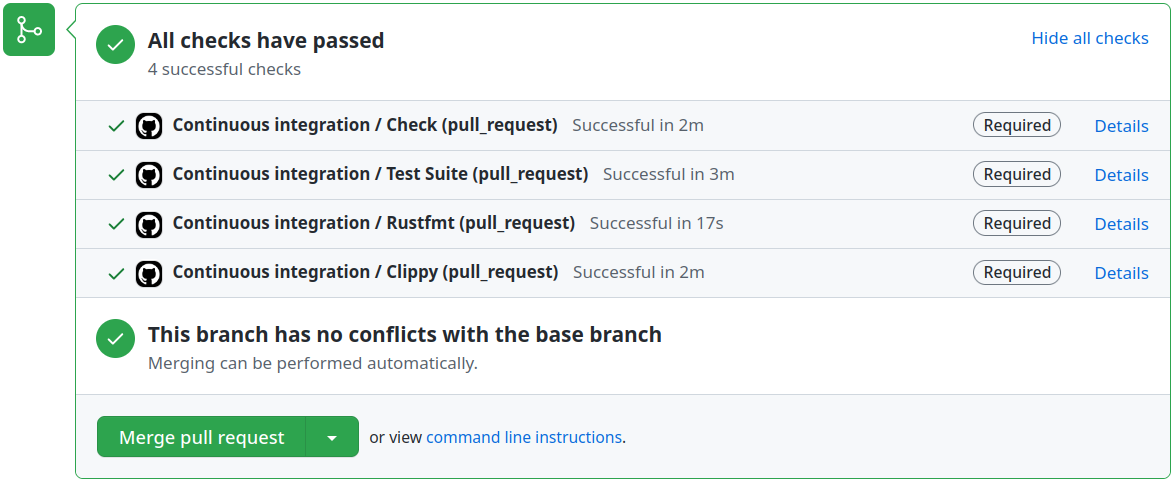
\includegraphics[width=\linewidth]{ci-pr-success}
\caption{Screenshot of a Pull Request where all checks finished successfully}
\end{figure}

\section{Language Design}

\subsection{Primitive types}
By default, Craft comes with some built-in (primitive), data types. These are
the following:

\begin{itemize}
    \item \textbf{i64:} 64 bit integer
    \item \textbf{f64:} 64 bit float
    \item \textbf{string:} array of characters
    \item \textbf{bool:} boolean
\end{itemize}

\subsection{Start of the program}
The starting point of craft programs is at the main function.

\begin{code}
fn main() {
    printf("Hello World!\n");
}
\end{code}

\subsection{Functions}
As you can see from the previous snippet, functions are declared with the fn
keyword, followed by its name, and  the parameters between parenthesis. The
parameters are declared by specifing the identifier, followed by a colon and the
type of the parameter. The return type comes after the closing parenthesis of
the parameters. The braces that suround the body of the function are always
mandatory.

\begin{code}
    fn something(a: i64, b: i64) i64 { ... }
\end{code}

\subsubsection{Variable declaration}
Variables are declared with the keyword \texttt{let}. The type of the variable
is infered from the value.

\begin{code}
let four = 2 + 2; // type inferred to be an integer
let four = 2.0 + 2.0; // type inferred to be float
\end{code}

Variables are \textbf{immutable by default}, which means that once initialized
their value cannot be changed. They act like constants that can be initialized
at runtime. If the variable needs to be mutated, it can, but only by adding the
keyword \textit{mut} after \textit{let}. So for example the following snippet
would fail to compile:

\begin{code}
    fn main() {
        let i = 0;
        i = i + 1; // compile error, variable is not mutable!
    }
\end{code}

The correct way to do it would be like this:

\begin{code}
    fn main() {
        let mut i = 0;
        i = i + 1; // compiles just fine, variable is mutable
    }
\end{code}

This design choice comes from the idea that a lot of bugs come from 
mutating variables when we don't actually want to. By making them immutable by
default, the user has to make the conscious choice of telling the compiler that
he/she wants to mutate the variable. This way, if he/she mutates a variable that
didn't intend to mutate, the compiler will catch it.

\subsection{Loops and control flow}
The way to repeat instructions multiple times in Craft is by using while loops.
They can be used like this:
\begin{code}
    let mut i = 0;
    while i < 100 {
        // do stuff
        i = i + 1;
    }
\end{code}

Another way to repeat instructions is by using recursion:
\begin{code}
fn fib(n: i64) i64 {
    if n <= 1 {
        n
    } else {
        fib(n - 1) + fib(n - 2)
    }
}
\end{code}

Apart from loops, we also have if statements to create branches in our code. 
They can be used like so:

\begin{code}
    if a > b {
        // do stuff
    } else if a == b {
        // do other stuff
    } else {
        // do other stuff
    }
\end{code}

Notice that in both if and while statements, parenthesis around the conditional 
expression are not necessary. They can still be used if the programmer desires
but the idiomatic way to do it is without parenthesis since it's easier to read 
and type.

\subsection{Expressions and statements}
Craft is an expression based language, which means that most constructs in the
language are expressions. An expression is a valid unit of code that evaluates
to a value. So for example, 2+2 is an expression, since it evaluates to a value
(4 in this case). On the other hand we have statements, which don't evaluate to
a value. For example, (\texttt{let a = 2+2;} is a statement that contains the 2
+ 2 expression, but the value is captured by the variable 'a', thus it's not
returned, and it becomes a statement. Usually statements end in semicolon,
except special cases like for example loops.

So when we said that Craft is expression based, it means that pretty much
everything returns a value. For example if statements, are not actually
statements, but expressions. We can do something like this:

\begin{code}
    let max = if a >= b { a } else { b };
\end{code}

In the code snippet above we are assigning the value returned from the if
expression to a variable. We can do that, because the last item in each of the
branches of the if expression is returning an expression (of the same type in
both branches, else it's a compile time error). Whenever the last expression in
a code block (anything surrounded by curly braces) does not contain a semicolon,
it means that block will return the value of evaluating that expression. So this
actually works: 

\begin{code}
    let four = {
        2 + 2
    };

    let x = {
        let x = func();
        x
    }
\end{code}

The block ends in an expression without semicolon, thus it returns the value of
evaluating that expression (4) and assigns that to the variable. This works for 
functions too:

\begin{code}
    fn add(a: i64, b: i64) i64 {
        a + b
    }

    fn max(a: i64, b: i64) i64 {
        if a >= b { a } else { b }
    }
\end{code}

If we were to add a semicolon to any of the return expressions on the previous
functions, we would get a compilation error, since we would turn the expressions
into statements, and the function would not return anything.

It's important to note that \textit{if} expressions \textbf{must} have an else
branch, since a value always has to be returned from the expression. If it's 
used as a statement (it doesn't return a value), then it's fine to have only the
\textit{if} branch.

Since blocks return values they can also be used for grouping expressions. For
example, we can change the precedence of arithmetic operations using blocks:

\begin{code}
    let a =  2 * { 3 + 2 }; // a will equal 10
\end{code}

What the previous code does is: it evaluates 2, then evaluates the block which
returns 5, and then multiplies both expressions.

\subsubsection{Examples of expressions}
\begin{code}
// function calls
func()
// arithmetic operations
2 + 2 
// if else
if x != y { x } else { y }
// binary comparisons
x > y 
// code blocks
{ expr }
\end{code}

\subsubsection{Examples of statements}
\begin{code}
let a = 2 + 2;  // variable declaration
while true {  } // loops
if a > b { printf("hello world"); } // ifs without return expr.
\end{code}

\subsection{Return statements}
We talked about blocks returning values by leaving the last expression without
semicolon. So if we want a function to return a value we just leave the last
expression of the function without semicolon, and it will be returned. But what
if you need to return earlier, maybe based on some condition? For those cases
there's the return statement, which instantly returns from the function when
called. It can be invoked with the \textbf{\textit{ret}} keyword. For example,
when implementing a recursive Fibonacci, we could do it like this:

\begin{code}
fn fib(n: i64) i64 {
    if n <= 1 {
        ret n;
    }
    fib(n - 1) + fib(n - 2)
}
\end{code}

\subsection{Data structures}
We talked about some primitive data types, but that's not always enough to model
more complex programs. That's why we can define custom data structures using 
structs. Structs work the same way they do in other languages like C or Rust.
We declare them like this:

\begin{code}
struct User {
    name: string
    age: i64
}
\end{code}

When creating an instance of a struct we do it the following way:

\begin{code}
    let user = User!{
        name: "Tux",
        age: 27,
    };
\end{code}

\subsection{Arrays}
Craft has support for arrays. They are fixed size and can be declared like this:

\begin{code}
let a = [1, 2, 3] i64;
\end{code}

The type annotations for an array follow the pattern \texttt{[type; size]}. 
For example, when declaring a function that takes an int array of three elements
as a parameter and returns that same array:

\begin{code}
fn do_nothing(arr: [i64; 3]) [i64; 3] {
    arr
}
\end{code}

Whenever we want to access an element of an array we use square brackets with 
the index of the element we want to access. Arrays in Craft are zero indexed, 
meaning the index of the first element is 0.

\begin{code}
let a = [1, 2, 3] i64;
let b = 2 + a[0]; // b = 3
\end{code}

\subsection{Print statements}
In order to print to stdout with Craft, the printf statement can be used. It
works the same way as printf in C (it actually calls libc under the hood).

\begin{code}
    let x = 2 + 2;
    printf("This is 2 + 2 => %d\n", x);
\end{code}

\subsection{Naming conventions}
In Craft function and variable names are written in snake\_case. It's 
only structs that are written in PascalCase.

\section{Tech Stack}

Writing a compiler does not require many tools, but some of them can help a lot
in paving the road. For this compiler we are going to mainly use two tools: 
The Rust Programming Language and LLVM.

\subsection{Rust}
Rust is a systems programming language that was first released in 2010. It was
developed by the Mozilla Foundation with the goal of creating a safe and
concurrent language that would be suitable for low-level systems programming
tasks, such as operating systems, and performance critical programs, like a
browser engine. One of the major features of the language is it's guaranteed
memory-safety (and thread-safety) without requiring the use of a garbage
collector or reference counting (and thus not compromising on performance).
This combined with its powerful type system, helps catch a lot of bugs at 
compile-time.

For this reason we are going to use this language. It's also really comfortable
to use and comes with a lot of great tooling like cargo, which is the command 
line tool used for compiling, managing dependencies, etc. and clippy, a linter
that comes built in and gives great hints on how to improve the code.

\subsection{LLVM}
LLVM is a toolchain for building compilers, i.e. a set of tools that help us
implementing compilers. It was created in 2003 by Chris Lattner (also creator of
the Swift programming language) and has the support of companies like Apple
(LLVM is an integral part of XCode and Swift for iOS application development),
Google, IBM or Intel \cite{sponsors}. Currently, there are several mainstream programming
languages that use it, such as C and C++ (via the Clang compiler), Rust, Swift,
Crystal...

As we said LLVM has a lot of tools, but among all them, the LLVM Core libraries
are the most important and particularly relevant for us. We will be referring to 
them as LLVM from now on for simplicity. 

LLVM will allow us to generate assembly for a lot of different architectures
and apply many optimizations to the code without any extra effort. It can even
generate Web Assembly, which allows us to run the language in modern web
browsers. The Craft compiler will generate LLVM IR (Intermidiete
Representation), and then it will be piped to LLVM, which will take the IR,
apply transformations to it, in order to optimize it, and then the assembly for
the target architecture will be generated.

Generating LLVM IR instead of assembly, also frees us from some headaches. For
example, since LLVM is architecture independent, when we generate the code, we
don't need to worry about the number of registers, as we have an unlimited
number of virtual registers, which LLVM will later map to the registers of the
corresponding architecture.

As we discussed, LLVM also applies optimizations to the generated code, like
dead code elimination, constant folding, loop unrolling, etc. However, in order
for LLVM to perform these optimizations, we will have to generate the code in
SSA form (Static Single-Assignment). This means that we can only assign a value
to a variable once. If we need to reassign a value, a new variable has to be
created that replaces the other one. The reason SSA is used is that it makes
applying optimizations a lot easier.

We will explore LLVM in more detail later in the article.

\section{Architecture}
Most compilers are divided into two parts: the front-end and the back-end. The
front-end is the part of the compilers that takes the source code and transforms
it into an intermediate representation than will later be transformed into the
actual machine code by the back-end. In our case, since we are using LLVM, we
don't need to worry too much about the back-end, since LLVM will be in charge of
generating the machine code. Our job will be to go from the source code to the
LLVM intermediate representation (we will call it \textbf{\textit{IR}} from now
on). The front-end of the compiler is typically composed of four main steps:
lexical analysis (implemented by the lexer), syntactic analysis (implemented by
the parser), semantic analysis and the intermediate code generation.

\begin{figure}[ht]
\centering
\captionsetup{justification=centering,margin=1cm}
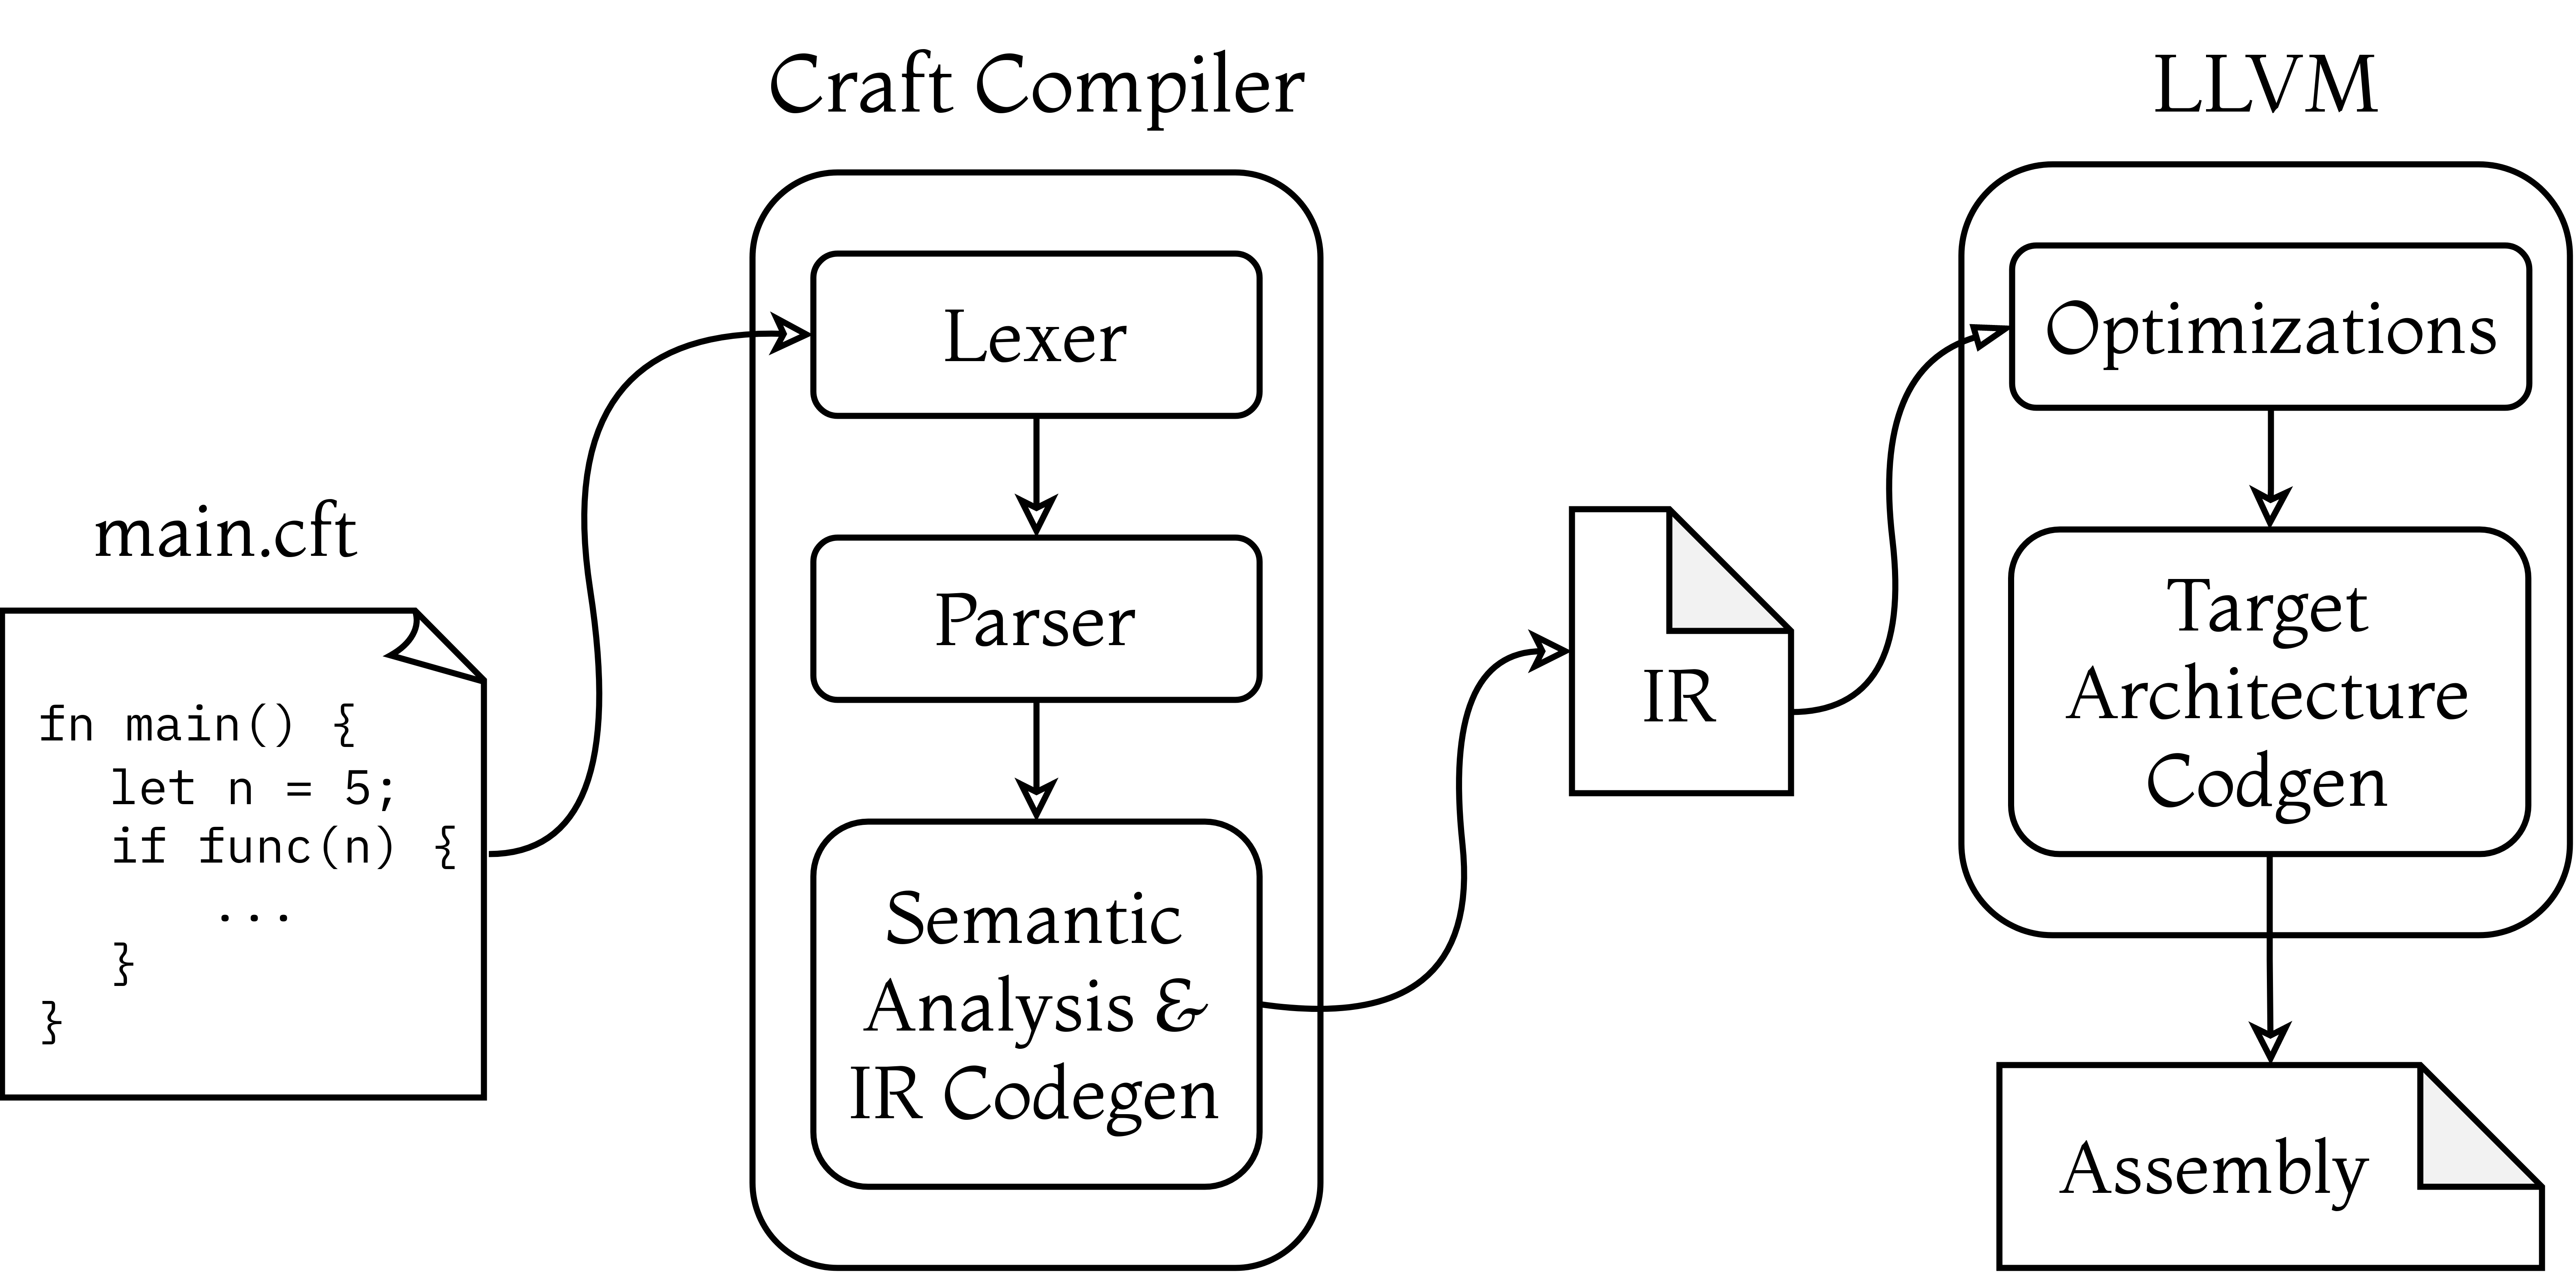
\includegraphics[width=\linewidth]{arch}
\caption{Diagram showing the compilation workflow of a Craft program}
\end{figure}

\subsection{Lexer} 
This step consists of breaking the source code into a sequence of tokens. A
token is a basic building block of the languages, such as a keyword or an
identifier.

A lexer can be implemented using an external lexical analyzer, but in our case
it will be implement by hand, since the goal is to learn how it works. 
Implementing a lexer from scratch is actually really simple. It works the 
following way:

\begin{enumerate}
    \item Start by reading the source code character by character until we reach
        the end.
    \item If the character by itself forms a valid sequence (e.g. a parenthesis)
        we create a token from it. If it doesn't, we continue reading characters
        until we find a valid sequence and then create the token.
\end{enumerate}

Note that sometimes we may find a valid sequence, but that's not enough to
create a token, since it may be the start of another longer and valid sequence.
We may need to check the following character/s to check weather it continues. An
example of such case would be the '\texttt{>}' operator, since, by itself is a
valid sequence, but it may be the start of the '\texttt{>=}' operator. So we
need to check if the next character is an '\texttt{=}' or something else.

The lexer requires a bit of work to set up, but after that, expanding it is 
trivial, since we only need to add a new word to the list of reserved words, in 
the case we want to add a reserved word, or add a new rule that detects a new 
symbol for example.


\subsection{Parser}
The lexer allowed us to identify the symbols of the program, but it does not 
allow us to determine if their order is correct, or if they follow the rules of
the language (i.e. it's syntactically correct). That is the job of the parser.

The parser takes the sequence of tokens obtained from the lexer and
transforms it into an Abstract Syntax Tree (AST). This tree represents the
structure of the program and determines its syntactic structure. It will tell us
the order in which we need to execute the instructions.

To generate the AST, compilers use a context free grammar. A grammar is a set of
rules that tells us how to form valid strings of tokens in a specific language.
They are formed of a set of symbols, which can be divided into terminal and
non-terminal symbols, and a set of production rules that specify how the
non-terminal symbols can be replaced by sequences of terminal and non-terminal
symbols. A context free grammar is a type of grammar which rules do not depend
on the context in which the symbols appear.

The goal of the parser is to make the program obey the rules of the grammar.
Here's an example of a simple grammar for parsing function prototypes:

\begin{small}
\begin{verbatim}

<proto>   ::= fn <id> "(" <params> ")"
<id>      ::= letter {letter | digit | "_"}
<params>  ::= "("{ <param> {, <param> } }")"
<param>   ::= <id>: <type>

\end{verbatim}
\end{small}

In the example above, the things between the \texttt{'<>'} are the productions,
and the things to the right of '::=' tell us how that rule is formed. For
example the proto production tells us that the prototype of a function is formed
by placing the fn keyword followed by an identifier (which is defined by the
\texttt{<id>} production), an opening parenthesis, the params (defined by the
\texttt{<params>} production) and a closing parenthesis. The curly braces 
indicate that the contents they surround can be repeated zero or more times. 
If the braces had quotes (i.e. "\{") then that would mean that we expect to have 
an actual curly brace on the code.

\vspace{10px}

Translating the grammar to actual code is actually quite simple, it's almost a
literal translation by implementing a recursive descent parser. If we were to
translate the proto rule to code, it would look something like this:
\vfill

\begin{code}
fn parse_prototype() -> (Prototype, Err) {
    // we expect to find the fn keyword,
    // else it's an error
    match current_token().kind {
        // The advance function moves to the next token
        TokenKind::Fn => advance(),
        _ => return Err("Expected fn keyword"),
    };

    // we expect to find the function name,
    // else it's an error
    let name = match current_token().kind {
        TokenKind::Identifier => current_token().lexeme,
        _ => return Err("Expected an identifier"),
    };

    advance();

    // we call the params rule
    let params = parse_params();

    // we are done, we return a struct 
    // with the info of the prototype
    return Prototype { 
        name,
        params,
    };
}
\end{code}

\subsection{Semantic Analysis and [IR] Code Generation}
Once we have an AST, we can traverse it to generate the LLVM IR. Since this is a
simple compiler, we are going to do the semantic analysis in this step. With 
more complex compilers, we may want to create a specific step of semantic 
analysis, but in our case it is not necessary. Semantic analysis basically 
checks things like if a variable exists when referencing it, or if the type of a
variable is correct (for example if we are multiplying an integer with a struct,
the semantic analyzer will catch it and throw a compilation error).

LLVM has the concept of modules. A module contains all the information
associated with one code file. If we have multiple files, we simply have to
create different modules and link them. Modules contain functions and functions
are made up of blocks. Blocks are defined by specifying a label. These labels
are like assembly labels, they define sections within out code, and we can use
them to make jumps to the different sections. Blocks are made up of
instructions, similar to the instructions we find in assembly.

\begin{figure}[ht]
\centering
\captionsetup{justification=centering,margin=1cm}
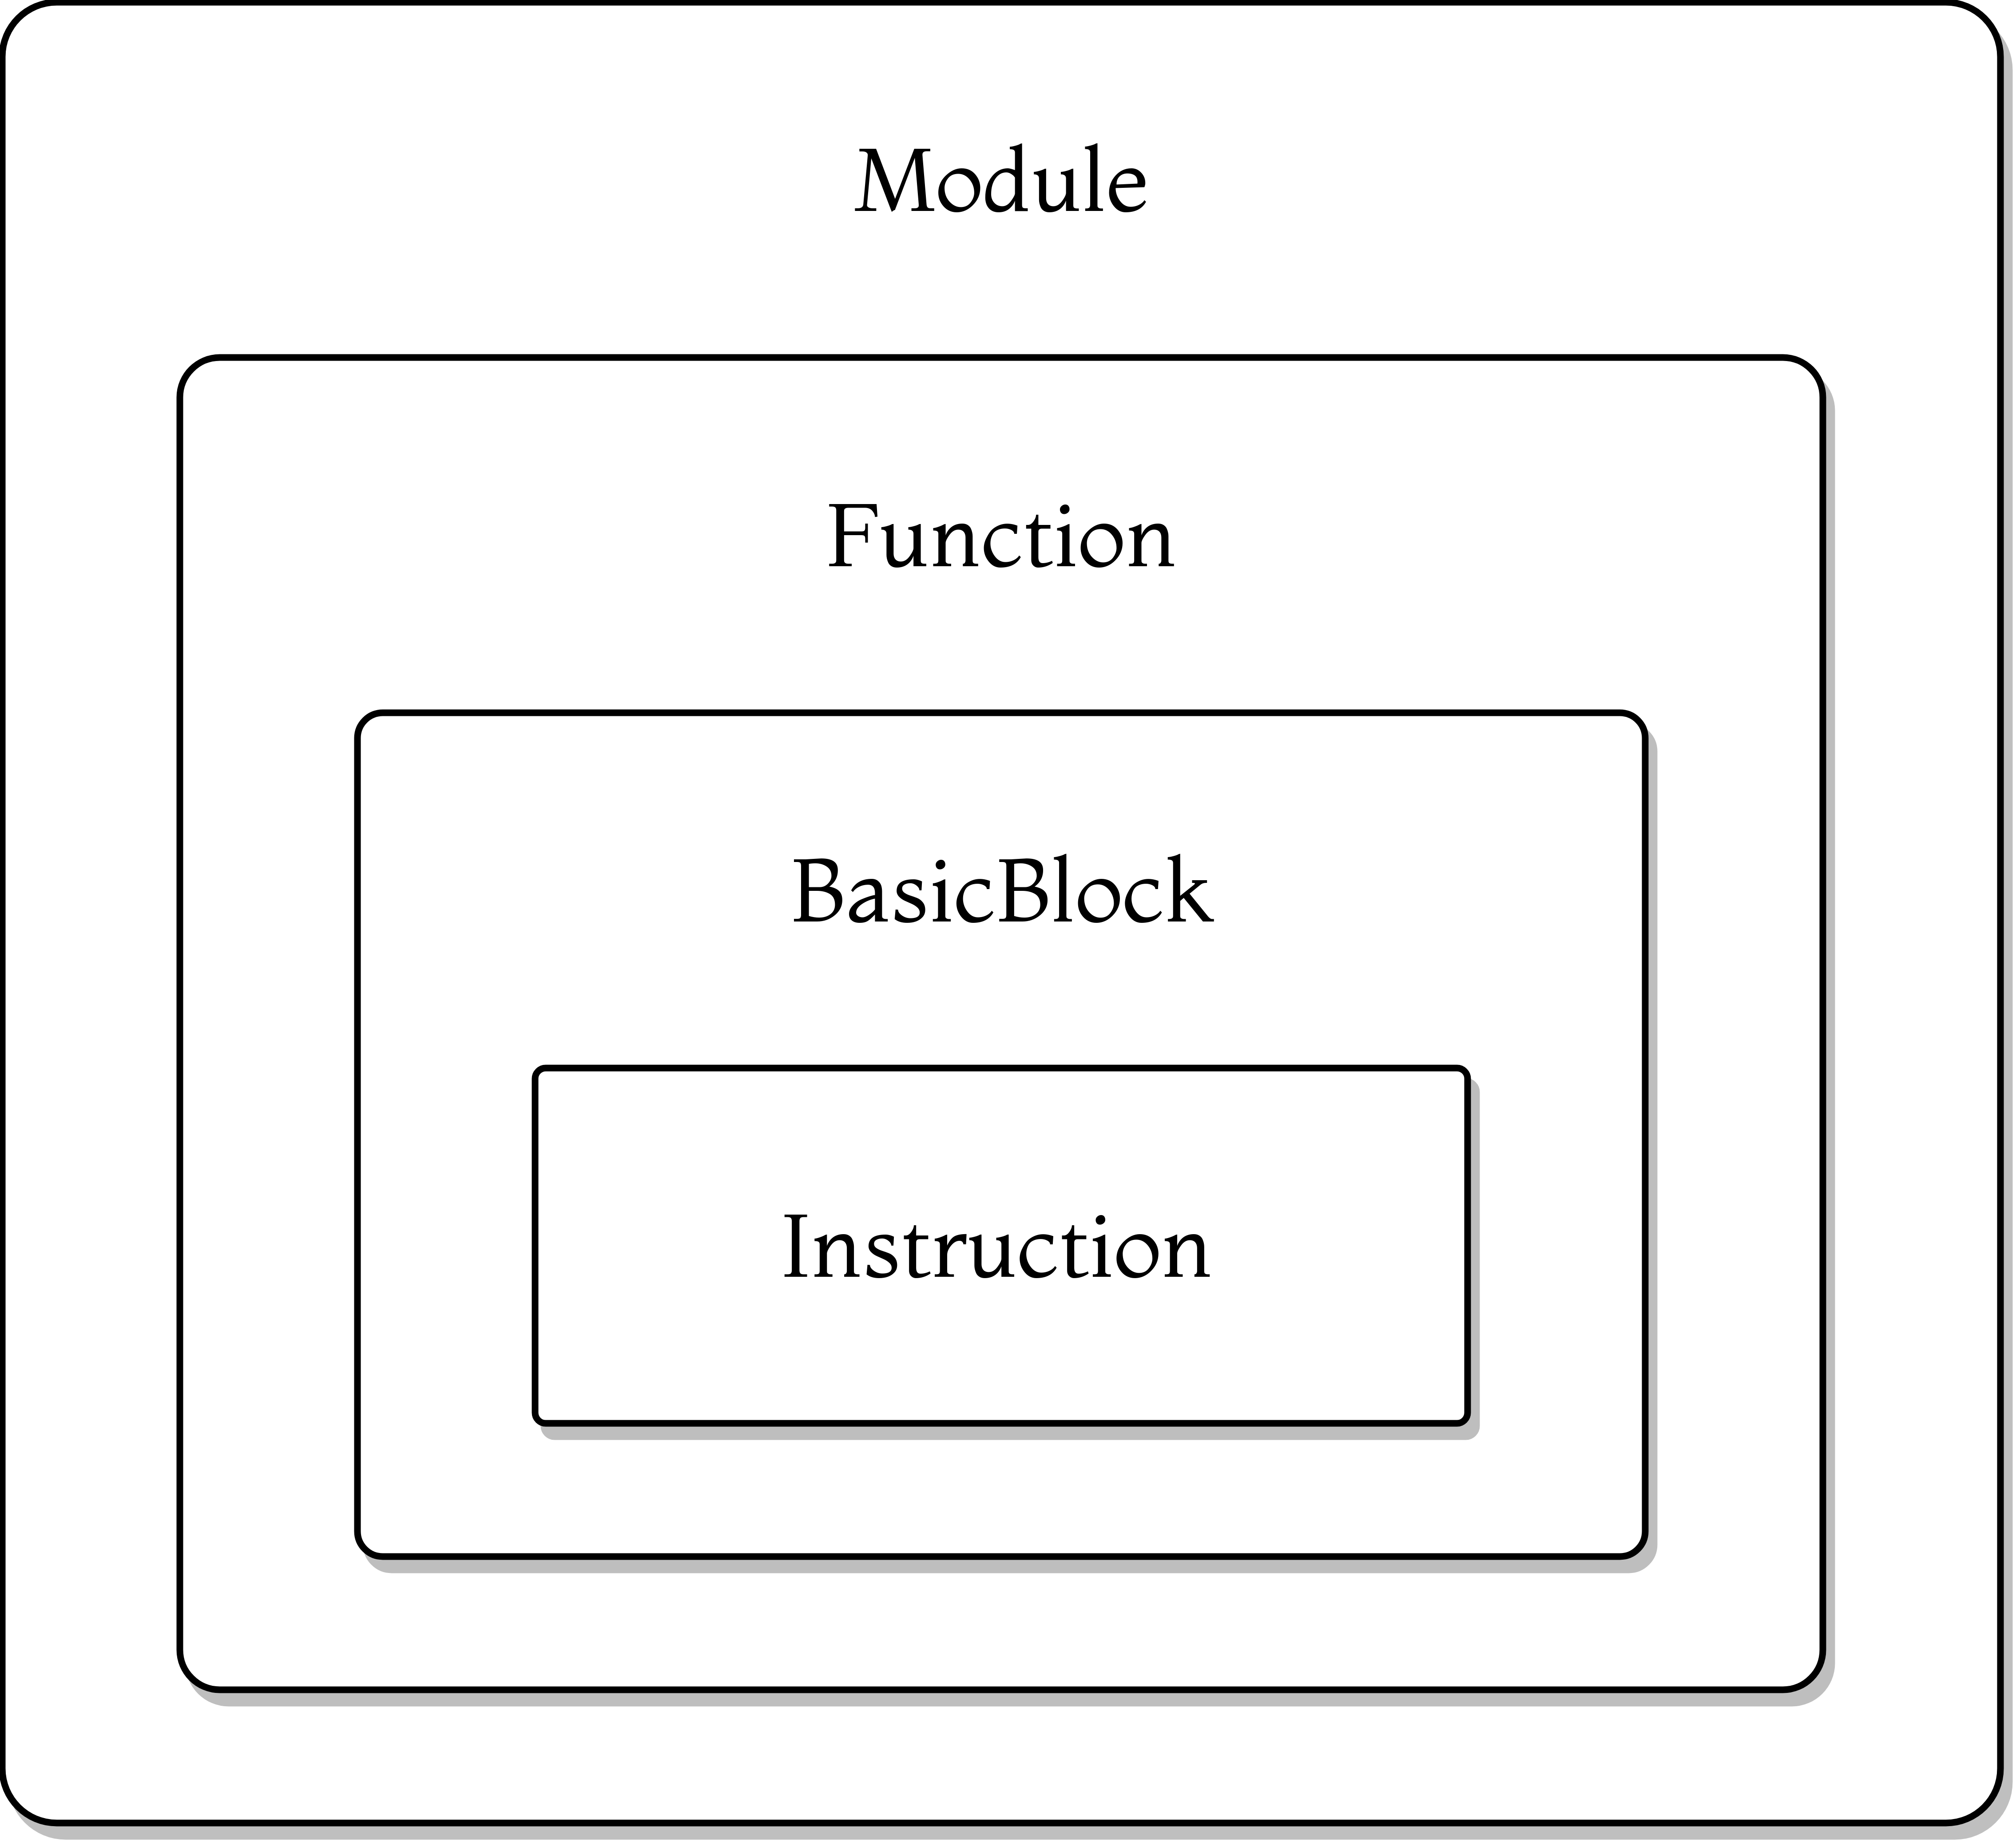
\includegraphics[width=0.65\linewidth]{llvm-blocks}
\caption{Overview of the different building blocks of LLVM}
\end{figure}

Let's see an example of a small piece of code and what it would look like in the
intermediate representation of LLVM. We have the following function that
receives two integers and returns the maximum:

\begin{code}
fn max(int a, int b) int {
    if a > b { a } else { b }
}
\end{code}

If we translate it to LLVM IR we have the following code:

\begin{code}
define i32 @max(i32 %a, i32 %b) {
entry:
  %0 = icmp sgt i32 %a, %b
  br i1 %0, label %btrue, label %bfalse

btrue:
  br label %end

bfalse:
  br label %end

end:
  %retval = phi i32 [%a, %btrue], [%b, %bfalse]
  ret i32 %retval
}
\end{code}

The first line of the previous code defines a function, which receives two
32 bits integers. A label entry is defined below.

The first thing it does, on the 'entry' tag, is comparing both integers (i.e.
the if condition). The \texttt{'sgt'} keyword \cite{sgt}, means 'signed greater
than', which, as the name says, does a greater than signed comparison. The
result of the comparison is a one bit integer which acts like a boolean. If it's
true, it will jump to the label \texttt{btrue}, otherwise to the label
\texttt{bfalse}.

In this case the two branches do the same thing: a jump to the label
\texttt{end}. There we come across a concept called phi nodes
\cite{phitutorial}\cite{phiinst}. The phi nodes are kind of an inverted if.
Depending on where we did the jump we will assign one value or another to the
variable \texttt{\%retval}. If we come from \texttt{btrue}, \texttt{\%retval} is
assigned \texttt{\%a}, and if we come from \texttt{bfalse} it is assigned to
\texttt{\%b}.

Now, why do the two branches jump to the \texttt{end} tag and then do a
conditional again in the \texttt{end} block? Couldn't we assign the value of
\texttt{retval} directly inside the branch \texttt{btrue} or \texttt{bfalse} and
spare us that third conditional? Well the answer is no, because then we would be
generating code that is not in SSA form (we would be assigning the value to
\%retval in two different places if we weren't using Phi nodes). And as we
mentioned earlier, LLVM requires the generated code to be in SSA form. And
that's why phi nodes exist, to be able to solve this kind of problem.

\subsubsection{LLVM API}

It's important to understand the LLVM IR, but generating all of that code by
hand is a lot of work, and it would require us to put a lot of infrastructure in
place. Fortunately, LLVM comes with a C++ API, that makes generating the IR a
lot easier. But there's a little problem, we are not using C++. Thankfully,
there's a Rust library called Inkwell \cite{inkwell}, that offers a comfortable
and idiomatic Rust interface to the LLVM API. Under the hood it calls the C++
API by using FFI (Foreign Function Interface).

The API is made of several entities. The most fundamental one is the
\textbf{\textit{BasicBlock}}, which represents the blocks that we find inside a
function, i.e. the set of instructions we find within a label. If we group a
bunch of BasicBlocks, we have an entity call \textbf{\textit{Function}}, which
represents a function in the IR. And by grouping a bunch of functions we get the
\textbf{\textit{Module}} entity. As you may notice these entities represent the
different parts that we saw when we talked about the IR.

Another important entity is \textit{\textbf{Context}}. We just need and instance of it, 
and it will keep track of the state of the compilation.

Finally, we have the \textit{\textbf{Builder}} entity, which is the one in charge of 
actually generating the code. For example, if we want to generate a comparison,
like the one we saw on the IR example, we would call the \textit{Builder}, 
telling it which instruction to generate:\\

\texttt{Builder.CreateICmpSGT(a, b, "some-name")}
\\

The first two parameters are the two values being compared. The third 
indicates the name of the generated variable (we can give it any name we want,
it's only useful for debugging).

The previous call will generate the following code (which is the third line of
the IR example we saw):

\texttt{\%0 = icmp sgt i32 \%a, \%b}

\section{Results}
The aim of this bachelor's thesis was to develop a programming language using
Rust and LLVM. The language was designed to incorporate basic features such as
if statements, while loops, functions, structs, and arrays.

The implementation of the language was carried out using Rust as the primary
programming language and LLVM as the compiler back-end. The use of Rust
allowed for a pleasant development experience and a fast compiler, while LLVM 
provided the necessary tools for code optimization and generation.

The final result of the project is a functioning programming language that
includes the aforementioned features and can be used to write and execute basic
programs. The implementation of the main features was successful, and the
language was able to perform as expected.

With the compiler as of today, we can write programs like the following:

\begin{code}
struct ComplexNum {
    real:      f64
    imaginary: f64
}

fn add(x: ComplexNum, y: ComplexNum) ComplexNum {
    ComplexNum!{
        real: x.real + y.real,
        imaginary: x.imaginary + y.imaginary,
    }
}

fn main() {
    let x = ComplexNum!{
        real: 1.0,
        imaginary: 2.0,
    };

    let y = ComplexNum!{
        real: 3.0,
        imaginary: 4.0,
    };

    let z = add(x, y);
    printf("x + y = %f + %fi\n", z.real, z.imaginary);
}
\end{code}

Or this which prints an approximation of the Mandelbrot set:

\begin{code}
fn mandelbrot(a: f64, b: f64) f64 {
    let mut za = 0.0;
    let mut zb = 0.0;

    let mut i = 0;

    while i < 50 {
        za = (za*za - zb*zb) + a;
        zb = (za*zb + za*zb) + b;
        i = i+1;
    }

    za*za + zb*zb
}

fn main() {
    let xstart = -2.0;
    let xend = 0.5;
    let ystart = 1.0;
    let yend = -1.0;

    let xstep = 0.0315;
    let ystep = -0.05;

    let mut x = xstart;
    let mut y = ystart;

    while y > yend {
        x = xstart;
        while x < xend {
            if mandelbrot(x, y) < 4.0 {
                printf("x");
            } else {
                printf(" ");
            }
            x = x + xstep; 
        }
        printf("\n");
        y = y + ystep;
    };
}
\end{code}

The output of this program can be found on the appendix \ref{appendix:a}.

Furthermore, the project provided an opportunity to gain experience in using
Rust and LLVM, as well as to gain a deeper understanding of the design and
implementation of programming languages. The combination of Rust and LLVM proved
to be a powerful combination for developing a compiler.

\section{Conclusions and future work}
The development of a programming language is a long and arduous process. It
requires the work of a lot of very good engineers, and a lot of time. The goal
of this project was not to create a production ready language packed with
features and an extensive standard library, but rather to create a simple
language with the basic functionality to make something useful. It was a project
to learn about the internals of compilers and programming language design. And I
think the goal was accomplished. We have a simple language that allows us to
create programs that actually run. However, there are many opportunities for
future work and improvement, since, as stated, it takes a long time to develop a
good language:

\begin{itemize}
    \item \textbf{New features}: It would be interesting to add new features
        such as for loops with ranges, a pipe operator similar to the one in
        Elixir, list comprehension like in Python, and many more features that
        would make the development process a lot more pleasant.
    \item \textbf{Modules}: As of now, all code has to go on one file, there's
        no way to import code from another one. A module system has to be 
        designed and implemented in order to allow it.
    \item \textbf{Error handling mechanism}: Currently there's no way to handle
        errors. An error handling mechanism has to be put in place. The idea
        would be to use something similar to the error handling mechanism in 
        Rust, rather than exceptions, since it gives the code linearity, and 
        they have to be explicitly handled on each case.
    \item \textbf{Tooling}: Some extra tooling like a formatter or a linter
        could be included with the compiler.
\end{itemize}

\renewcommand\refname{References}
\begin{thebibliography}{11}
\bibitem{rustsafety} Stanford CS 242: Programming Languages. \textit{Memory safety in Rust}. Accessed the 6th of February 2023. Available at: \url{https://stanford-cs242.github.io/f18/lectures/05-1-rust-memory-safety.html}
\bibitem{gocodegen}Go compiler. \textit{Generating machine code}. Accessed the 6th of February 2023. Available at: \url{https://github.com/golang/go/blob/master/src/cmd/compile/README.md#7-generating-machine-code}
\bibitem{rustllvm} Guide to Rustc development. \textit{Code generation}. Accessed the 6th of February 2023. Available at: \url{https://rustc-dev-guide.rust-lang.org/backend/codegen.html}
\bibitem{clangllvm} Clang compiler. Accessed the 6th of February 2023. Available at: \url{https://clang.llvm.org}
\bibitem{kotlininterop} \textit{Calling Java from Kotlin}. Accessed the 6th of February 2023. Available at: \url{https://kotlinlang.org/docs/java-interop.html}
\bibitem{elixirinterop} \textit{Erlang libraries from Elixir}. Accessed the 6th of February 2023. Available at: \url{https://elixir-lang.org/getting-started/erlang-libraries.html}
\bibitem{repo} \textit{Craft Git Repository}. Accessed the 6th of February 2023. Available at: \\\url{https://github.com/josepmdc/craft}
\bibitem{sponsors} LLVM Foundation sponsors. Accessed the 7th of February 2023. Available at: \url{https://foundation.llvm.org/docs/sponsors/}
\bibitem{sgt} LLVM Language Reference. \textit{icmp instruction}. Accessed the 7th of February 2023. Available at: \url{https://llvm.org/docs/LangRef.html#icmp-instruction}
\bibitem{phitutorial} LLVM tutorial \textit{LLVM IR for if/then/else}. Accessed the 7th of February 2023. Available at: \url{https://llvm.org/docs/tutorial/MyFirstLanguageFrontend/LangImpl05.html#llvm-ir-for-if-then-else}
\bibitem{phiinst} LLVM Language Reference. \textit{phi instruction}. Accessed the 7th of February 2023. Available at: \url{https://llvm.org/docs/LangRef.html#phi-instruction}
\bibitem{inkwell} \textit{Inkwell Documentation}. Accessed the 4th of October 2023. Available at: \\\url{https://thedan64.github.io/inkwell/inkwell/index.html}
\end{thebibliography}

\renewcommand\refname{Bibliography}
\begin{thebibliography}{11}
\bibitem{ci} Nystrom, R. \textit{Crafting Interpreters}. Published July 2021. ISBN 0990582930.
\bibitem{compilergo} Ball, T. \textit{Writing A Compiler In Go}. Published August 2018. ISBN 398201610X.
\bibitem{llvmtut} \textit{LLVM Kaleidoscope Tutorial: Implementing a Language with LLVM}. Accessed the 25th of October 2022. Available at: \url{https://llvm.org/docs/tutorial}
\bibitem{llvm4plc} Rathi, M. \textit{A complete guide to LLVM for programming language creators}. Mukuls Blogs. Accessed the 2nd of November 2022. Available at: \\\url{https://mukulrathi.com/create-your-own-programming-language/llvm-ir-cpp-api-tutorial}
\bibitem{mhlctllvm} \textit{Mapping High Level Constructs to LLVM IR}. Accessed the 20th of October 2022. Available at: \\\url{https://mapping-high-level-constructs-to-llvm-ir.readthedocs.io/en/latest/README.html}
\end{thebibliography}

\newpage
\appendix

\section*{Appendix}

\setcounter{section}{1}

\subsection{Output of the Mandelbrot set program}
\label{appendix:a}
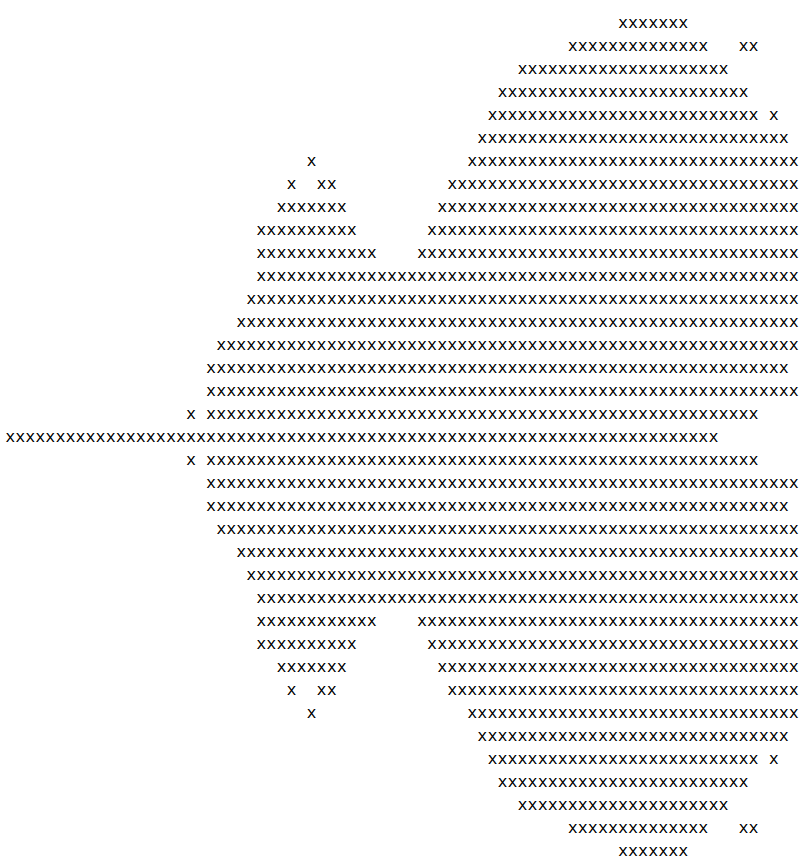
\includegraphics[width=\linewidth]{mandelbrot}

\end{document}
